
\subsection*{1.}

Parmi les enfants buvant une boisson sucrée ou plus par jour, un enfant sur 8 est en surpoids, donc :
\[
p_B(S) = \frac{1}{8} = \frac{125}{8 \times 125} = \frac{125}{1000} = 0{,}125.
\]

\subsection*{2.}

\begin{center}
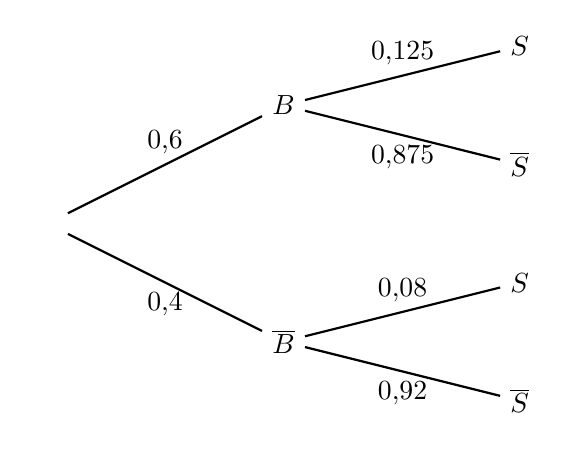
\begin{tikzpicture}[thick, scale=1.5]
\node (P_-1_0) at (-2,-1.5) {$\phantom{A}$};
\node (P_0_0) at (0,-0.5) {$B$};
\draw (P_-1_0) -- (P_0_0) node[midway, above] {$0{,}6$};
\node (P_1_0) at (2,-0) {$S$};
\draw (P_0_0) -- (P_1_0) node[midway, above] {$0{,}125$};
\node (P_1_1) at (2,-1) {$\overline{S}$};
\draw (P_0_0) -- (P_1_1) node[midway, below] {$0{,}875$};
\node (P_0_2) at (0,-2.5) {$\overline{B}$};
\draw (P_-1_0) -- (P_0_2) node[midway, below] {$0{,}4$};
\node (P_1_2) at (2,-2) {$S$};
\draw (P_0_2) -- (P_1_2) node[midway, above] {$0{,}08$};
\node (P_1_3) at (2,-3) {$\overline{S}$};
\draw (P_0_2) -- (P_1_3) node[midway, below] {$0{,}92$};
\end{tikzpicture}
\end{center}

\subsection*{3.}

\(p(B \cap S) = p(B) \times p_B(S) = 0{,}6 \times 0{,}125 = 0{,}075\).

\subsection*{4.}

De même, on a :
\[
p(\overline{B} \cap S) = p(\overline{B}) \times p_{\overline{B}}(S) = 0{,}4 \times 0{,}08 = 0{,}032.
\]
D'après la loi des probabilités totales :
\[
p(S) = p(B \cap S) + p(\overline{B} \cap S) = 0{,}075 + 0{,}032 = 0{,}107.
\]

\subsection*{5.}

On a :
\[
p_S(B) = \frac{p(S \cap B)}{p(S)} = \frac{0{,}075}{0{,}107} \approx 0{,}7009,
\]
soit  \( 0{,}701 \) au millième près.

